\color{black}
\subsection{Specifica componenti Model::Core::Feature}
\label{specificaModelCoreAlgorithm}

\begin{figure}[!h]
\centering
			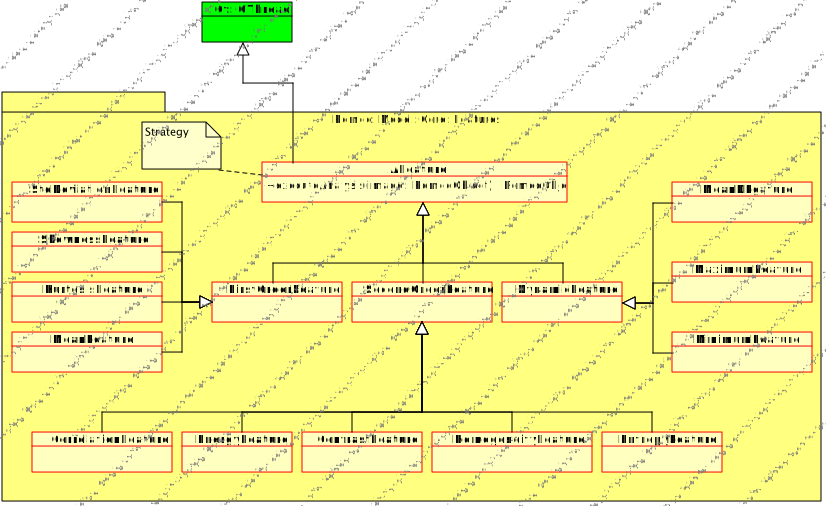
\includegraphics[scale=0.6]{../Specifica_Tecnica/Content/Immagini/Romeo__Model__Core__Adapters__Features.png}
			\caption{Diagramma package \textsl{Romeo::Model::Core::Feature}}
			\label{romeo_model_core}
\end{figure}

Package\g{} contenente le classi per le feature\g{}.

% % % % % % % % % % % % % % % % % % % % % %
% % % % % % % % % % % % % % % % % % % %
\subsubsection{AFeature (abstract)}
\label{afeature}
\begin{figure}[!h]
\centering
			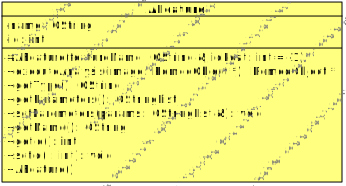
\includegraphics[scale=1]{./Content/Immagini/modelCore/AFeature.png}
			\caption{Diagramma classe \textsl{AFeature}}
			\label{feature_img}
\end{figure}

\paragraph{Descrizione \\} Classe astratta che rappresenta una generica feature\g{}. Definisce dei contratti per l'esecuzione degli algoritmi, che dovranno essere implementati dalle sue sottoclassi. Rappresenta la componente Strategy dell'omonimo design pattern\g{}.

\paragraph{Utilizzo\\} Fornisce i metodi per l'esecuzione di una feature\g{} su un immagine bidimensionale o tridimensionale.

\paragraph{Eredita da}
\begin{itemize}
	\item Qt::QThread
\end{itemize}

\paragraph{\textcolor{black}{Attributi\\}}
	\begin{itemize}
		\item \color{teal}\verb!- name : QString !
		\color{black}
		\subparagraph{Descrizione:} stringa contenente il nome della feature\g{}.
		\item \color{teal}\verb!- id : int !
		\color{black}
		\subparagraph{Descrizione:} intero contentente il codice identificativo della feature\g{}.
	\end{itemize}

\paragraph{\textcolor{black}{Metodi\\}}
	\begin{itemize}
	\item \color{blue}\verb! # AFeature(featureName : const QString & , id :	int)!
		\color{black}
		\subparagraph{Descrizione:} costruttore della classe AFeature.
		\subparagraph{Argomenti}
			\begin{itemize}
				\item \color{RoyalPurple} \verb!name : const QString &! \\ 
				\color{black} nome della feature\g{}.	
				\item \color{RoyalPurple} \verb!id : int! \\ 
				\color{black} codice identificativo della feature\g{}.	
			\end{itemize}
			
	\item \color{blue}\verb! + executeAnalysis(image : RomeoObject *) : RomeoObject *!
		\color{black}
		\subparagraph{Descrizione:} metodo puro che esegue la feature su un dato e ritorna il dato di output.
		\subparagraph{Argomenti}
			\begin{itemize}
				\item \color{RoyalPurple} \verb!image : RomeoObject * ! \\ 
				\color{black} dato in ingresso alla feature.		
			\end{itemize}
		\subparagraph{Note}
			\begin{itemize}
				\item il metodo deve essere marcato virtuale puro.
			\end{itemize}
			
	\item \color{blue}\verb! + getType() : QString !
		\color{black}
		\subparagraph{Descrizione:}  contratto per restituire il tipo della feature\g{}.
		\subparagraph{Note}
			\begin{itemize}
				\item deve essere marcato costante.
			\end{itemize}
			
	\item \color{blue}\verb! + getParameters() : QStringList!
		\color{black}
		\subparagraph{Descrizione:}  contratto per restituisce una lista di stringe, contenente la lista degli 						attributi.
		\subparagraph{Note}
			\begin{itemize}
				\item deve essere marcato costante.
			\end{itemize}
	
	\item \color{blue}\verb! + setParameters(params : const QStringList &) : void !
		\color{black}
		\subparagraph{Descrizione:} inserisce i parametri della feature\g{}.
		\subparagraph{Argomenti}
			\begin{itemize}
				\item \color{RoyalPurple} \verb!params : const QStringList & ! \\ 
				\color{black} lista di parametri della feature.		
			\end{itemize}
		\subparagraph{Note}
			\begin{itemize}
				\item il metodo deve essere marcato virtuale.
			\end{itemize}
		
	\item \color{blue}\verb! + getName() : QString!
		\color{black}
		\subparagraph{Descrizione:} restituisce il nome della feature\g{}.
		\subparagraph{Note}
			\begin{itemize}
				\item deve essere marcato costante.
			\end{itemize}
			
	\item \color{blue}\verb! + getId() : int!
		\color{black}
		\subparagraph{Descrizione:} restituisce il codice identificativo della feature\g{}.
		\subparagraph{Note}
			\begin{itemize}
				\item deve essere marcato costante.
			\end{itemize}
			
	\item \color{blue}\verb! + setId(i : int) : void!
		\color{black}
		\subparagraph{Descrizione:} inserisce il codice identificativo della feature.
		\subparagraph{Argomenti}
			\begin{itemize}
				\item \color{RoyalPurple} \verb!params : const QStringList & ! \\ 
				\color{black} codice identificativo della feature.		
			\end{itemize}

	\end{itemize}
	

% % % % % % % % % % % % % % % % % % % % % % % % % % % % % % % % %
% % % % % % FIRST ORDER FEATURE % % % % % % % % % % % % % % % % % % % % % %
% % % % % % % % % % % % % % % % % % % % % % % % % % % % % %
\color{black}
\pagebreak
\subsubsection{FirstOrderFeature (abstract)}
\label{FirstOrderFeature}
\begin{figure}[!h]
\centering
			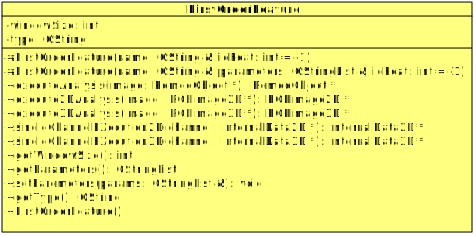
\includegraphics[scale=1]{./Content/Immagini/modelCore/FirstOrderFeature.png}
			\caption{Diagramma classe \textsl{FirstOrderFeature}}
			\label{FirstOrderFeature_img}
\end{figure}

\paragraph{Descrizione \\} Classe astratta che rappresenta una generica feature\g{} del primo ordine. Deriva da AFeature e rimane astratta perché non implementa i contratti di quest'ultima. Le sue sottoclassi rappresenteranno le componenti ConcreteStrategy del design pattern\g{} Strategy.

\paragraph{Utilizzo\\} Viene utilizzata durante un'analisi recuperare le informazioni sulla dimensione della finestra, la lista dei parametri e il tipo della feature\g{}.

\paragraph{Eredita da:}
\begin{itemize}
	\item AFeature.
\end{itemize}

\paragraph{\textcolor{black}{Attributi\\}}
	\begin{itemize}
		\item \color{teal}\verb!- windowSize : int!
		\color{black}
		\subparagraph{Descrizione:} dimensione della finestra sulla quale effettuare le operazioni.
		\item \color{teal}\verb!- type : QString!
		\color{black}
		\subparagraph{Descrizione:} specifica il tipo della feature\g{}.
	\end{itemize}

\paragraph{\textcolor{black}{Metodi\\}}
	\begin{itemize}
	\item \color{blue}\verb! # FirstOrderFeature(name : QString & , idFeat : int)!
		\color{black}
		\subparagraph{Descrizione:} costruttore della classe FirstOrderFeature.
		\subparagraph{Argomenti}
			\begin{itemize}
				\item \color{RoyalPurple} \verb!name : QString &! \\ 
				\color{black} Nome della feature. Viene passato al costruttore della superclasse.	
				\item \color{RoyalPurple} \verb!id : int! \\ 
				\color{black} codice identificativo della feature\g{}.	
			\end{itemize}
			
	\item \color{blue}\verb! # FirstOrderFeature(name : QString &, parameters : QStringList & , id : int)!
		\color{black}
		\subparagraph{Descrizione:} Costruttore a tre parametri della classe. Richiama il costruttore della 						superclasse.
		\subparagraph{Argomenti}
			\begin{itemize}
				\item \color{RoyalPurple} \verb!name : QString &! \\ 
				\color{black} Nome della feature. Viene passato al costruttore della superclasse.	
				\item \color{RoyalPurple} \verb!parameters : QStringList &! \\ 
				\color{black} Lista contenente i parametri della feature\g{}. Verrà effettuato il \textit{parsing} 						della lista, dalla quale verrà estratta la dimensione della finestra.
				\item \color{RoyalPurple} \verb!id : int! \\ 
				\color{black} codice identificativo della feature\g{}.	
			\end{itemize}
			
	\item \color{blue}\verb! + executeAnalysis(image : RomeoObject *) : RomeoObject *!
		\color{black}
		\subparagraph{Descrizione:} metodo puro che esegue la feature su un dato e ritorna il dato di output.
		\subparagraph{Argomenti}
			\begin{itemize}
				\item \color{RoyalPurple} \verb!image : RomeoObject * ! \\ 
				\color{black} dato in ingresso alla feature.		
			\end{itemize}
		\subparagraph{Note}
			\begin{itemize}
				\item il metodo deve essere marcato virtuale.
			\end{itemize}
						
	\item \color{blue}\verb! + execute2DAnalysis(image : RGBImage2D *) : RGBImage2D *!
		\color{black}
		\subparagraph{Descrizione:} metodo puro che esegue la feature su un immagine 2D e ritorna un immagine 2D 						processata.
		\subparagraph{Argomenti}
			\begin{itemize}
				\item \color{RoyalPurple} \verb!image : RGBImage2D * ! \\ 
				\color{black} immagine 2D in ingresso alla feature.		
			\end{itemize}
		\subparagraph{Note}
			\begin{itemize}
				\item il metodo deve essere marcato virtuale.
			\end{itemize}
			
	\item \color{blue}\verb! + execute3DAnalysis(image : RGBImage3D *) : RGBImage3D *!
		\color{black}
		\subparagraph{Descrizione:} metodo puro che esegue la feature su un immagine 3D e ritorna un immagine 3D 						processata.
		\subparagraph{Argomenti}
			\begin{itemize}
				\item \color{RoyalPurple} \verb!image : RGBImage3D * ! \\ 
				\color{black} immagine 3D in ingresso alla feature.		
			\end{itemize}
		\subparagraph{Note}
			\begin{itemize}
				\item il metodo deve essere marcato virtuale.
			\end{itemize}
			
	\item \color{blue}\verb! + singleChannelEXecution2D(channel : InternalData2D *) : InternalData2D *!
		\color{black}
		\subparagraph{Descrizione:} metodo puro che esegue la feature su un canale di un immagine 2D.
		\subparagraph{Argomenti}
			\begin{itemize}
				\item \color{RoyalPurple} \verb!channel : InternalData2D * ! \\ 
				\color{black} canale di un immagine 2D in ingresso alla feature.		
			\end{itemize}
		\subparagraph{Note}
			\begin{itemize}
				\item il metodo deve essere marcato virtuale puro.
			\end{itemize}
			
	\item \color{blue}\verb! + singleChannelEXecution3D(channel : InternalData3D *) : InternalData3D *!
		\color{black}
		\subparagraph{Descrizione:} metodo puro che esegue la feature su un canale di un immagine 3D.
		\subparagraph{Argomenti}
			\begin{itemize}
				\item \color{RoyalPurple} \verb!channel : InternalData3D * ! \\ 
				\color{black} canale di un immagine 3D in ingresso alla feature.		
			\end{itemize}
		\subparagraph{Note}
			\begin{itemize}
				\item il metodo deve essere marcato virtuale puro.
			\end{itemize}
			
	\item \color{blue}\verb! + getWindowSize() : int!
		\color{black}
		\subparagraph{Descrizione:} metodo che ritorna la dimensione della finestra .
		\subparagraph{Note}
			\begin{itemize}
				\item il metodo deve essere marcato costante.
			\end{itemize}
			
	\item \color{blue}\verb! + getParameters() : QStringList!
		\color{black}
		\subparagraph{Descrizione:} metodo che ritorna la lista dei parametri della feature\g{} .
		\subparagraph{Note}
			\begin{itemize}
				\item il metodo deve essere marcato virtuale.
			\end{itemize}
			
	\item \color{blue}\verb! + setParameters(params : const QStringList &) : void!
		\color{black}
		\subparagraph{Descrizione:} inserisce i parametri della feature\g{}.
		\subparagraph{Argomenti}
			\begin{itemize}
				\item \color{RoyalPurple} \verb!params : const QStringList & ! \\ 
				\color{black} lista di parametri della feature.		
			\end{itemize}
		\subparagraph{Note}
			\begin{itemize}
				\item il metodo deve essere marcato virtuale.
			\end{itemize}
			
	\item \color{blue}\verb! + getType() : QString!
		\color{black}
		\subparagraph{Descrizione:} metodo che ritorna il tipo della feature\g{} .
		\subparagraph{Note}
			\begin{itemize}
				\item il metodo deve essere marcato costante.
				\item il metodo deve essere marcato virtuale.
			\end{itemize}
			
	\end{itemize}


% % % % % % % % % % % % % % % % % % % % % % % % % % % % % % % % %
% % % % % % SECOND ORDER FEATURE% % % % % % % % % % % % % % % % % % % % % % %
% % % % % % % % % % % % % % % % % % % % % % % % % % % % % %
\color{black}
\pagebreak
\subsubsection{SecondOrderFeature (abstract)}
\label{SecondOrderFeature}
\begin{figure}[!h]
\centering
			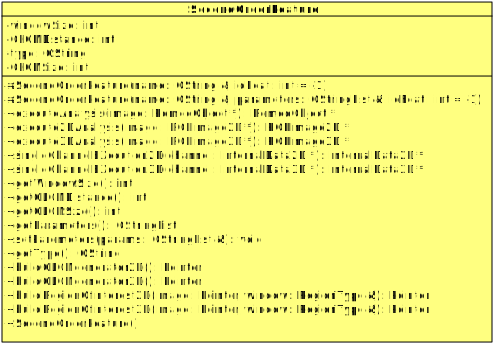
\includegraphics[scale=1]{./Content/Immagini/modelCore/SecondOrderFeature.png}
			\caption{Diagramma classe \textsl{SecondOrderFeature}}
			\label{SecondOrder_img}
\end{figure}

\paragraph{Descrizione \\} Classe astratta che rappresenta una generica feature\g{} del secondo ordine. Deriva da AFeature e rimane astratta perché non implementa i contratti di quest'ultima. Le sue sottoclassi rappresenteranno le componenti ConcreteStrategy del design pattern\g{} Strategy.

\paragraph{Utilizzo\\} Viene utilizzata durante un'analisi recuperare le informazioni della feature\g{}, la lista dei parametri e il tipo della feature\g{}.

\paragraph{Eredita da:}
\begin{itemize}
	\item AFeature.
\end{itemize}

\paragraph{\textcolor{black}{Attributi\\}}
	\begin{itemize}
		\item \color{teal}\verb!- windowSize : int!
		\color{black}
		\subparagraph{Descrizione:} dimensione della finestra sulla quale effettuare le operazioni.
		\item \color{teal}\verb!- type : QString!
		\color{black}
		\subparagraph{Descrizione:} specifica il tipo della feature\g{}.
		\item \color{teal}\verb!- GLCMSize : int!
		\color{black}
		\subparagraph{Descrizione:} specifica la dimensione della matrice GLCM.
		\item \color{teal}\verb!- GLCMDistance : int!
		\color{black}
		\subparagraph{Descrizione:} specifica la distanza della matrice GLCM.
	\end{itemize}

\paragraph{\textcolor{black}{Metodi\\}}
	\begin{itemize}
	\item \color{blue}\verb! # SecondOrderFeature(name : QString & , idFeat : int)!
		\color{black}
		\subparagraph{Descrizione:} costruttore della classe SecondOrderFeature.
		\subparagraph{Argomenti}
			\begin{itemize}
				\item \color{RoyalPurple} \verb!name : QString &! \\ 
				\color{black} Nome della feature. Viene passato al costruttore della superclasse.	
				\item \color{RoyalPurple} \verb!id : int! \\ 
				\color{black} codice identificativo della feature\g{}.	
			\end{itemize}
			
	\item \color{blue}\verb! # SecondOrderFeature(name : QString &, parameters : QStringList & , id : int)!
		\color{black}
		\subparagraph{Descrizione:} Costruttore a tre parametri della classe. Richiama il costruttore della 						superclasse.
		\subparagraph{Argomenti}
			\begin{itemize}
				\item \color{RoyalPurple} \verb!name : QString &! \\ 
				\color{black} Nome della feature. Viene passato al costruttore della superclasse.	
				\item \color{RoyalPurple} \verb!parameters : QStringList &! \\ 
				\color{black} Lista contenente i parametri della feature\g{}. Verrà effettuato il \textit{parsing} 						della lista, dalla quale verrà estratta la dimensione della finestra.
				\item \color{RoyalPurple} \verb!id : int! \\ 
				\color{black} codice identificativo della feature\g{}.	
			\end{itemize}
			
	\item \color{blue}\verb! + executeAnalysis(image : RomeoObject *) : RomeoObject *!
		\color{black}
		\subparagraph{Descrizione:} metodo puro che esegue la feature su un dato e ritorna il dato di output.
		\subparagraph{Argomenti}
			\begin{itemize}
				\item \color{RoyalPurple} \verb!image : RomeoObject * ! \\ 
				\color{black} dato in ingresso alla feature.		
			\end{itemize}
		\subparagraph{Note}
			\begin{itemize}
				\item il metodo deve essere marcato virtuale.
			\end{itemize}
						
	\item \color{blue}\verb! + execute2DAnalysis(image : RGBImage2D *) : RGBImage2D *!
		\color{black}
		\subparagraph{Descrizione:} metodo puro che esegue la feature su un immagine 2D e ritorna un immagine 2D 						processata.
		\subparagraph{Argomenti}
			\begin{itemize}
				\item \color{RoyalPurple} \verb!image : RGBImage2D * ! \\ 
				\color{black} immagine 2D in ingresso alla feature.		
			\end{itemize}
		\subparagraph{Note}
			\begin{itemize}
				\item il metodo deve essere marcato virtuale.
			\end{itemize}
			
	\item \color{blue}\verb! + execute3DAnalysis(image : RGBImage3D *) : RGBImage3D *!
		\color{black}
		\subparagraph{Descrizione:} metodo puro che esegue la feature su un immagine 3D e ritorna un immagine 3D 						processata.
		\subparagraph{Argomenti}
			\begin{itemize}
				\item \color{RoyalPurple} \verb!image : RGBImage3D * ! \\ 
				\color{black} immagine 3D in ingresso alla feature.		
			\end{itemize}
		\subparagraph{Note}
			\begin{itemize}
				\item il metodo deve essere marcato virtuale.
			\end{itemize}
			
	\item \color{blue}\verb! + singleChannelEXecution2D(channel : InternalData2D *) : InternalData2D *!
		\color{black}
		\subparagraph{Descrizione:} metodo puro che esegue la feature su un canale di un immagine 2D.
		\subparagraph{Argomenti}
			\begin{itemize}
				\item \color{RoyalPurple} \verb!channel : InternalData2D * ! \\ 
				\color{black} canale di un immagine 2D in ingresso alla feature.		
			\end{itemize}
		\subparagraph{Note}
			\begin{itemize}
				\item il metodo deve essere marcato virtuale puro.
			\end{itemize}
			
	\item \color{blue}\verb! + singleChannelEXecution3D(channel : InternalData3D *) : InternalData3D *!
		\color{black}
		\subparagraph{Descrizione:} metodo puro che esegue la feature su un canale di un immagine 3D.
		\subparagraph{Argomenti}
			\begin{itemize}
				\item \color{RoyalPurple} \verb!channel : InternalData3D * ! \\ 
				\color{black} canale di un immagine 3D in ingresso alla feature.		
			\end{itemize}
		\subparagraph{Note}
			\begin{itemize}
				\item il metodo deve essere marcato virtuale puro.
			\end{itemize}
			
	\item \color{blue}\verb! + getWindowSize() : int!
		\color{black}
		\subparagraph{Descrizione:} metodo che ritorna la dimensione della finestra .
		\subparagraph{Note}
			\begin{itemize}
				\item il metodo deve essere marcato costante.
			\end{itemize}
			
	\item \color{blue}\verb! + getGLCMDistance() : int!
		\color{black}
		\subparagraph{Descrizione:} metodo che ritorna la distanza della matrice GLCM	.
		\subparagraph{Note}
			\begin{itemize}
				\item il metodo deve essere marcato costante.
			\end{itemize}
			
	\item \color{blue}\verb! + getGLCMSize() : int!
		\color{black}
		\subparagraph{Descrizione:} metodo che ritorna la dimensione della matrice GLCM	.
		\subparagraph{Note}
			\begin{itemize}
				\item il metodo deve essere marcato costante.
			\end{itemize}
			
			
	\item \color{blue}\verb! + getParameters() : QStringList!
		\color{black}
		\subparagraph{Descrizione:} metodo che ritorna la lista dei parametri della feature\g{} .
		\subparagraph{Note}
			\begin{itemize}
				\item il metodo deve essere marcato virtuale.
			\end{itemize}
			
	\item \color{blue}\verb! + setParameters(params : const QStringList &) : void!
		\color{black}
		\subparagraph{Descrizione:} inserisce i parametri della feature\g{}.
		\subparagraph{Argomenti}
			\begin{itemize}
				\item \color{RoyalPurple} \verb!params : const QStringList & ! \\ 
				\color{black} lista di parametri della feature.		
			\end{itemize}
		\subparagraph{Note}
			\begin{itemize}
				\item il metodo deve essere marcato virtuale.
			\end{itemize}
			
	\item \color{blue}\verb! + getType() : QString!
		\color{black}
		\subparagraph{Descrizione:} metodo che ritorna il tipo della feature\g{} .
		\subparagraph{Note}
			\begin{itemize}
				\item il metodo deve essere marcato costante.
				\item il metodo deve essere marcato virtuale.
			\end{itemize}
			
			
	\item \color{blue}\verb! + buildGLCMgenerator2D() : InternalData2D::ImageToGlcmType::Pointer !
		\color{black}
		\subparagraph{Descrizione:} costruisce l'oggetto che si occupa del calcolo della GLCM per le immagini 2D.
		
	\item \color{blue}\verb! + buildGLCMgenerator3D() : InternalData3D::ImageToGlcmType::Pointer !
		\color{black}
		\subparagraph{Descrizione:} costruisce l'oggetto che si occupa del calcolo della GLCM per le immagini 3D.
		
	\item \color{blue}\verb! + buildRegionOfInterest2D(image : InternalData2D::ImageType::Pointer , !\\																	\verb!window : InternalData2D::ImageType::RegionType &) !\\
													\verb!: InternalData2D::roiType::Pointer  !					
		\color{black}
		\subparagraph{Descrizione:} costruisce la regione di iterazione per le immagini 2D.
		\subparagraph{Argomenti}
			\begin{itemize}
				\item \color{RoyalPurple} \verb!image : InternalData2D::ImageType::Pointer ! \\ 
				\color{black} immagine in input.		
			\end{itemize}
			\begin{itemize}
				\item \color{RoyalPurple} \verb!window : InternalData2D::ImageType::RegionType & ! \\ 
				\color{black} regione dell'immagine da scorrere.		
			\end{itemize}
			
	\item \color{blue}\verb! + buildRegionOfInterest3D(image : InternalData3D::ImageType::Pointer , !\\																	\verb!window : InternalData3D::ImageType::RegionType &) !\\
													\verb!: InternalData3D::roiType::Pointer  !					
		\color{black}
		\subparagraph{Descrizione:} costruisce la regione di iterazione per le immagini 3D.
		\subparagraph{Argomenti}
			\begin{itemize}
				\item \color{RoyalPurple} \verb!image : InternalData3D::ImageType::Pointer ! \\ 
				\color{black} immagine in input.		
			\end{itemize}
			\begin{itemize}
				\item \color{RoyalPurple} \verb!window : InternalData3D::ImageType::RegionType & ! \\ 
				\color{black} regione dell'immagine da scorrere.		
			\end{itemize}
		
	\end{itemize}

% % % % % % % % % % % % % % % % % % % % % % % % % % % % % % % % %
% % % % % % DYNAMIC FEATURE% % % % % % % % % % % % % % % % % % % % % % %
% % % % % % % % % % % % % % % % % % % % % % % % % % % % % %
\color{black}
\pagebreak
\subsubsection{DynamicFeature (abstract)}
\label{DynamicFeature}
\begin{figure}[!h]
\centering
			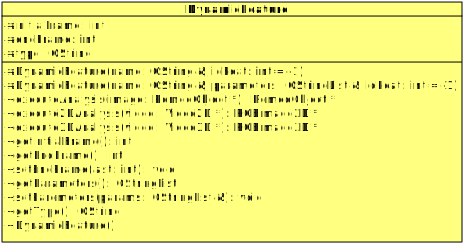
\includegraphics[scale=1]{./Content/Immagini/modelCore/DynamicFeature.png}
			\caption{Diagramma classe \textsl{DynamicFeature}}
			\label{Dynamic_img}
\end{figure}

\paragraph{Descrizione \\} Classe astratta che rappresenta una generica feature\g{} dinamica. Deriva da AFeature e rimane astratta perché non implementa i contratti di quest'ultima. Le sue sottoclassi rappresenteranno le componenti ConcreteStrategy del design pattern\g{} Strategy.

\paragraph{Utilizzo\\} Viene utilizzata durante un'analisi recuperare la lista dei parametri e il tipo della feature\g{}.

\paragraph{Eredita da:}
\begin{itemize}
	\item AFeature.
\end{itemize}

\paragraph{\textcolor{black}{Attributi\\}}
	\begin{itemize}
		\item \color{teal}\verb!- type : QString!
		\color{black}
		\subparagraph{Descrizione:} specifica il tipo della feature\g{}.
		\item \color{teal}\verb!- initialFrame : int!
		\color{black}
		\subparagraph{Descrizione:} specifica il frame d'inizio del video.
		\item \color{teal}\verb!- endFrame : int!
		\color{black}
		\subparagraph{Descrizione:} specifica l'ultimo frame del video.
	\end{itemize}

\paragraph{\textcolor{black}{Metodi\\}}
	\begin{itemize}
	\item \color{blue}\verb! # DynamicFeature(name : QString & , idFeat : int)!
		\color{black}
		\subparagraph{Descrizione:} costruttore della classe SecondOrderFeature.
		\subparagraph{Argomenti}
			\begin{itemize}
				\item \color{RoyalPurple} \verb!name : QString &! \\ 
				\color{black} Nome della feature. Viene passato al costruttore della superclasse.	
				\item \color{RoyalPurple} \verb!id : int! \\ 
				\color{black} codice identificativo della feature\g{}.	
			\end{itemize}
			
	\item \color{blue}\verb! # DynamicFeature(name : QString &, parameters : QStringList & , id : int)!
		\color{black}
		\subparagraph{Descrizione:} Costruttore a tre parametri della classe. Richiama il costruttore della 						superclasse.
		\subparagraph{Argomenti}
			\begin{itemize}
				\item \color{RoyalPurple} \verb!name : QString &! \\ 
				\color{black} Nome della feature. Viene passato al costruttore della superclasse.	
				\item \color{RoyalPurple} \verb!parameters : QStringList &! \\ 
				\color{black} Lista contenente i parametri della feature\g{}. Verrà effettuato il \textit{parsing} 						della lista, dalla quale verrà estratta la dimensione della finestra.
				\item \color{RoyalPurple} \verb!id : int! \\ 
				\color{black} codice identificativo della feature\g{}.	
			\end{itemize}
			
	\item \color{blue}\verb! + executeAnalysis(image : RomeoObject *) : RomeoObject *!
		\color{black}
		\subparagraph{Descrizione:} metodo puro che esegue la feature su un dato e ritorna il dato di output.
		\subparagraph{Argomenti}
			\begin{itemize}
				\item \color{RoyalPurple} \verb!image : RomeoObject * ! \\ 
				\color{black} dato in ingresso alla feature.		
			\end{itemize}
		\subparagraph{Note}
			\begin{itemize}
				\item il metodo deve essere marcato virtuale.
			\end{itemize}
						
	\item \color{blue}\verb! + execute2DAnalysis(image : RGBImage2D *) : RGBImage2D *!
		\color{black}
		\subparagraph{Descrizione:} metodo puro che esegue la feature su un immagine 2D e ritorna un immagine 2D 						processata.
		\subparagraph{Argomenti}
			\begin{itemize}
				\item \color{RoyalPurple} \verb!image : RGBImage2D * ! \\ 
				\color{black} immagine 2D in ingresso alla feature.		
			\end{itemize}
		\subparagraph{Note}
			\begin{itemize}
				\item il metodo deve essere marcato virtuale.
			\end{itemize}
			
	\item \color{blue}\verb! + execute3DAnalysis(image : RGBImage3D *) : RGBImage3D *!
		\color{black}
		\subparagraph{Descrizione:} metodo puro che esegue la feature su un immagine 3D e ritorna un immagine 3D 						processata.
		\subparagraph{Argomenti}
			\begin{itemize}
				\item \color{RoyalPurple} \verb!image : RGBImage3D * ! \\ 
				\color{black} immagine 3D in ingresso alla feature.		
			\end{itemize}
		\subparagraph{Note}
			\begin{itemize}
				\item il metodo deve essere marcato virtuale.
			\end{itemize}
			
	\item \color{blue}\verb! + getInitialFrame() : int!
		\color{black}
		\subparagraph{Descrizione:} metodo che ritorna l'indice del frame iniziale.
		\subparagraph{Note}
			\begin{itemize}
				\item il metodo deve essere marcato costante.
			\end{itemize}
			
	\item \color{blue}\verb! + getEndFrame() : int!
		\color{black}
		\subparagraph{Descrizione:} metodo che ritorna il frame finale.
		\subparagraph{Note}
			\begin{itemize}
				\item il metodo deve essere marcato costante.
			\end{itemize}
	
	\item \color{blue}\verb! + setEndFrame(last : int) : void!
		\color{black}
		\subparagraph{Descrizione:} metodo che inserisce l'indice dell'ultimo frame del video da considerare.
		\subparagraph{Argomenti}
			\begin{itemize}
				\item \color{RoyalPurple} \verb!last : int! \\ 
				\color{black} indice dell'ultimo frame del video da considerare.		
			\end{itemize}		
						
	\item \color{blue}\verb! + getParameters() : QStringList!
		\color{black}
		\subparagraph{Descrizione:} metodo che ritorna la lista dei parametri della feature\g{} .
		\subparagraph{Note}
			\begin{itemize}
				\item il metodo deve essere marcato virtuale.
			\end{itemize}
			
	\item \color{blue}\verb! + setParameters(params : const QStringList &) : void!
		\color{black}
		\subparagraph{Descrizione:} inserisce i parametri della feature\g{}.
		\subparagraph{Argomenti}
			\begin{itemize}
				\item \color{RoyalPurple} \verb!params : const QStringList & ! \\ 
				\color{black} lista di parametri della feature.		
			\end{itemize}
		\subparagraph{Note}
			\begin{itemize}
				\item il metodo deve essere marcato virtuale.
			\end{itemize}
			
	\item \color{blue}\verb! + getType() : QString!
		\color{black}
		\subparagraph{Descrizione:} metodo che ritorna il tipo della feature\g{} .
		\subparagraph{Note}
			\begin{itemize}
				\item il metodo deve essere marcato costante.
				\item il metodo deve essere marcato virtuale.
			\end{itemize}
		
	\end{itemize}


% % % % % % % % % % % % % % % % % % % % % % % % % % % % % % % % %
% % % % % % MEAN FEATURE % % % % % % % % % % % % % % % % % % % % % % %
% % % % % % % % % % % % % % % % % % % % % % % % % % % % % %
\color{black}
\pagebreak
\subsubsection{MeanFeature (class)}
\label{MeanFeature}
\begin{figure}[!h]
\centering
			\includegraphics[scale=1]{./Content/Immagini/modelCore/MeanFeature.png}
			\caption{Diagramma classe \textsl{MeanFeature}}
			\label{meanFeature_img}
\end{figure}

\paragraph{Descrizione \\} Classe che implementa la feature\g{} \textit{Mean}. Rappresenta la componente ConcreteStrategy del design pattern\g{} Strategy.
\\Per l'implementazione della feature\g{} il programmatore dovrà seguire l'appendice \ref{codicematlab}.

\paragraph{Utilizzo\\} Viene utilizzata durante un'analisi per applicare la feature\g{} a un \dataset{}.

\paragraph{Eredita da:}
\begin{itemize}
	\item FirstOrderFeature.
\end{itemize}

\paragraph{\textcolor{black}{Metodi\\}}
	\begin{itemize}
	\item \color{blue}\verb! # DynamicFeature(idFeat : int)!
		\color{black}
		\subparagraph{Descrizione:} costruttore della classe MeanFeature.
		\subparagraph{Argomenti}
			\begin{itemize}
				\item \color{RoyalPurple} \verb!id : int! \\ 
				\color{black} codice identificativo della feature\g{}.	
			\end{itemize}
			
	\item \color{blue}\verb! # DynamicFeature(parameters : QStringList & , id : int)!
		\color{black}
		\subparagraph{Descrizione:} Costruttore a due parametri della classe. Richiama il costruttore della 						superclasse.
		\subparagraph{Argomenti}
			\begin{itemize}	
				\item \color{RoyalPurple} \verb!parameters : QStringList &! \\ 
				\color{black} Lista contenente i parametri della feature\g{}. Verrà effettuato il \textit{parsing} 						della lista, dalla quale verrà estratta la dimensione della finestra.
				\item \color{RoyalPurple} \verb!id : int! \\ 
				\color{black} codice identificativo della feature\g{}.	
			\end{itemize}

	\item \color{blue}\verb! + singleChannelEXecution2D(channel : InternalData2D *) : InternalData2D *!
		\color{black}
		\subparagraph{Descrizione:} metodo puro che esegue la feature su un canale di un immagine 2D.
		\subparagraph{Argomenti}
			\begin{itemize}
				\item \color{RoyalPurple} \verb!channel : InternalData2D * ! \\ 
				\color{black} canale di un immagine 2D in ingresso alla feature.		
			\end{itemize}
		\subparagraph{Note}
			\begin{itemize}
				\item il metodo deve essere marcato virtuale puro.
			\end{itemize}
			
	\item \color{blue}\verb! + singleChannelEXecution3D(channel : InternalData3D *) : InternalData3D *!
		\color{black}
		\subparagraph{Descrizione:} metodo puro che esegue la feature su un canale di un immagine 3D.
		\subparagraph{Argomenti}
			\begin{itemize}
				\item \color{RoyalPurple} \verb!channel : InternalData3D * ! \\ 
				\color{black} canale di un immagine 3D in ingresso alla feature.		
			\end{itemize}
		\subparagraph{Note}
			\begin{itemize}
				\item il metodo deve essere marcato virtuale puro.
			\end{itemize}
			
	\end{itemize}



% % % % % % % % % % % % % % % % % % % % % % % % % % % % % % % % %
% % % % % % KURTOSIS FEATURE % % % % % % % % % % % % % % % % % % % % % % %
% % % % % % % % % % % % % % % % % % % % % % % % % % % % % %
\color{black}
\pagebreak
\subsubsection{KurtosisFeature (class)}
\label{KurtosisFeature}
\begin{figure}[!h]
\centering
			\includegraphics[scale=1]{./Content/Immagini/modelCore/KurtosisFeature.png}
			\caption{Diagramma classe \textsl{KurtosisFeature}}
			\label{kurtosisFeature_img}
\end{figure}

\paragraph{Descrizione \\} Classe che implementa la feature\g{} \textit{Kurtosis}. Rappresenta la componente ConcreteStrategy del design pattern\g{} Strategy.
\\Per l'implementazione della feature\g{} il programmatore dovrà seguire l'appendice \ref{codicematlab}.

\paragraph{Utilizzo\\} Viene utilizzata durante un'analisi per applicare la feature\g{} a un \dataset{}.

\paragraph{Eredita da:}
\begin{itemize}
	\item FirstOrderFeature.
\end{itemize}

\paragraph{\textcolor{black}{Metodi\\}}
	\begin{itemize}
	\item \color{blue}\verb! # DynamicFeature(idFeat : int)!
		\color{black}
		\subparagraph{Descrizione:} costruttore della classe MeanFeature.
		\subparagraph{Argomenti}
			\begin{itemize}
				\item \color{RoyalPurple} \verb!id : int! \\ 
				\color{black} codice identificativo della feature\g{}.	
			\end{itemize}
			
	\item \color{blue}\verb! # DynamicFeature(parameters : QStringList & , id : int)!
		\color{black}
		\subparagraph{Descrizione:} Costruttore a due parametri della classe. Richiama il costruttore della 						superclasse.
		\subparagraph{Argomenti}
			\begin{itemize}	
				\item \color{RoyalPurple} \verb!parameters : QStringList &! \\ 
				\color{black} Lista contenente i parametri della feature\g{}. Verrà effettuato il \textit{parsing} 						della lista, dalla quale verrà estratta la dimensione della finestra.
				\item \color{RoyalPurple} \verb!id : int! \\ 
				\color{black} codice identificativo della feature\g{}.	
			\end{itemize}

	\item \color{blue}\verb! + singleChannelEXecution2D(channel : InternalData2D *) : InternalData2D *!
		\color{black}
		\subparagraph{Descrizione:} metodo puro che esegue la feature su un canale di un immagine 2D.
		\subparagraph{Argomenti}
			\begin{itemize}
				\item \color{RoyalPurple} \verb!channel : InternalData2D * ! \\ 
				\color{black} canale di un immagine 2D in ingresso alla feature.		
			\end{itemize}
		\subparagraph{Note}
			\begin{itemize}
				\item il metodo deve essere marcato virtuale puro.
			\end{itemize}
			
	\item \color{blue}\verb! + singleChannelEXecution3D(channel : InternalData3D *) : InternalData3D *!
		\color{black}
		\subparagraph{Descrizione:} metodo puro che esegue la feature su un canale di un immagine 3D.
		\subparagraph{Argomenti}
			\begin{itemize}
				\item \color{RoyalPurple} \verb!channel : InternalData3D * ! \\ 
				\color{black} canale di un immagine 3D in ingresso alla feature.		
			\end{itemize}
		\subparagraph{Note}
			\begin{itemize}
				\item il metodo deve essere marcato virtuale puro.
			\end{itemize}
			
	\end{itemize}

% % % % % % % % % % % % % % % % % % % % % % % % % % % % % % % % %
% % % % % % SKEWNESS FEATURE % % % % % % % % % % % % % % % % % % % % % % %
% % % % % % % % % % % % % % % % % % % % % % % % % % % % % %
\color{black}
\pagebreak
\subsubsection{SkewnessFeature (class)}
\label{SkewnessFeature}
\begin{figure}[!h]
\centering
			\includegraphics[scale=1]{./Content/Immagini/modelCore/SkewnessFeature.png}
			\caption{Diagramma classe \textsl{SkewnessFeature}}
			\label{skewnessFeature_img}
\end{figure}

\paragraph{Descrizione \\} Classe che implementa la feature\g{} \textit{Skewness}. Rappresenta la componente ConcreteStrategy del design pattern\g{} Strategy.
\\Per l'implementazione della feature\g{} il programmatore dovrà seguire l'appendice \ref{codicematlab}.

\paragraph{Utilizzo\\} Viene utilizzata durante un'analisi per applicare la feature\g{} a un \dataset{}.

\paragraph{Eredita da:}
\begin{itemize}
	\item FirstOrderFeature.
\end{itemize}

\paragraph{\textcolor{black}{Metodi\\}}
	\begin{itemize}
	\item \color{blue}\verb! # DynamicFeature(idFeat : int)!
		\color{black}
		\subparagraph{Descrizione:} costruttore della classe SkewnessFeature.
		\subparagraph{Argomenti}
			\begin{itemize}
				\item \color{RoyalPurple} \verb!id : int! \\ 
				\color{black} codice identificativo della feature\g{}.	
			\end{itemize}
			
	\item \color{blue}\verb! # DynamicFeature(parameters : QStringList & , id : int)!
		\color{black}
		\subparagraph{Descrizione:} Costruttore a due parametri della classe. Richiama il costruttore della 						superclasse.
		\subparagraph{Argomenti}
			\begin{itemize}	
				\item \color{RoyalPurple} \verb!parameters : QStringList &! \\ 
				\color{black} Lista contenente i parametri della feature\g{}. Verrà effettuato il \textit{parsing} 						della lista, dalla quale verrà estratta la dimensione della finestra.
				\item \color{RoyalPurple} \verb!id : int! \\ 
				\color{black} codice identificativo della feature\g{}.	
			\end{itemize}

	\item \color{blue}\verb! + singleChannelEXecution2D(channel : InternalData2D *) : InternalData2D *!
		\color{black}
		\subparagraph{Descrizione:} metodo puro che esegue la feature su un canale di un immagine 2D.
		\subparagraph{Argomenti}
			\begin{itemize}
				\item \color{RoyalPurple} \verb!channel : InternalData2D * ! \\ 
				\color{black} canale di un immagine 2D in ingresso alla feature.		
			\end{itemize}
		\subparagraph{Note}
			\begin{itemize}
				\item il metodo deve essere marcato virtuale puro.
			\end{itemize}
			
	\item \color{blue}\verb! + singleChannelEXecution3D(channel : InternalData3D *) : InternalData3D *!
		\color{black}
		\subparagraph{Descrizione:} metodo puro che esegue la feature su un canale di un immagine 3D.
		\subparagraph{Argomenti}
			\begin{itemize}
				\item \color{RoyalPurple} \verb!channel : InternalData3D * ! \\ 
				\color{black} canale di un immagine 3D in ingresso alla feature.		
			\end{itemize}
		\subparagraph{Note}
			\begin{itemize}
				\item il metodo deve essere marcato virtuale puro.
			\end{itemize}
			
	\end{itemize}

% % % % % % % % % % % % % % % % % % % % % % % % % % % % % % % % %
% % % % % % STANDARD DEVIATION FEATURE % % % % % % % % % % % % % % % % % % % % % % %
% % % % % % % % % % % % % % % % % % % % % % % % % % % % % %
\color{black}
\pagebreak
\subsubsection{StandardDeviationFeature (class)}
\label{StandardDeviationFeature}
\begin{figure}[!h]
\centering
			\includegraphics[scale=1]{./Content/Immagini/modelCore/StandardDeviationFeature.png}
			\caption{Diagramma classe \textsl{StandardDeviationFeature}}
			\label{standardDeviationFeature_img}
\end{figure}

\paragraph{Descrizione \\} Classe che implementa la feature\g{} \textit{Standard Deviation}. Rappresenta la componente ConcreteStrategy del design pattern\g{} Strategy.
\\Per l'implementazione della feature\g{} il programmatore dovrà seguire l'appendice \ref{codicematlab}.

\paragraph{Utilizzo\\} Viene utilizzata durante un'analisi per applicare la feature\g{} a un \dataset{}.

\paragraph{Eredita da:}
\begin{itemize}
	\item FirstOrderFeature.
\end{itemize}


\paragraph{\textcolor{black}{Metodi\\}}
	\begin{itemize}
	\item \color{blue}\verb! # DynamicFeature(idFeat : int)!
		\color{black}
		\subparagraph{Descrizione:} costruttore della classe StandardDeviationFeature.
		\subparagraph{Argomenti}
			\begin{itemize}
				\item \color{RoyalPurple} \verb!id : int! \\ 
				\color{black} codice identificativo della feature\g{}.	
			\end{itemize}
			
	\item \color{blue}\verb! # DynamicFeature(parameters : QStringList & , id : int)!
		\color{black}
		\subparagraph{Descrizione:} Costruttore a due parametri della classe. Richiama il costruttore della 						superclasse.
		\subparagraph{Argomenti}
			\begin{itemize}	
				\item \color{RoyalPurple} \verb!parameters : QStringList &! \\ 
				\color{black} Lista contenente i parametri della feature\g{}. Verrà effettuato il \textit{parsing} 						della lista, dalla quale verrà estratta la dimensione della finestra.
				\item \color{RoyalPurple} \verb!id : int! \\ 
				\color{black} codice identificativo della feature\g{}.	
			\end{itemize}

	\item \color{blue}\verb! + singleChannelEXecution2D(channel : InternalData2D *) : InternalData2D *!
		\color{black}
		\subparagraph{Descrizione:} metodo puro che esegue la feature su un canale di un immagine 2D.
		\subparagraph{Argomenti}
			\begin{itemize}
				\item \color{RoyalPurple} \verb!channel : InternalData2D * ! \\ 
				\color{black} canale di un immagine 2D in ingresso alla feature.		
			\end{itemize}
		\subparagraph{Note}
			\begin{itemize}
				\item il metodo deve essere marcato virtuale puro.
			\end{itemize}
			
	\item \color{blue}\verb! + singleChannelEXecution3D(channel : InternalData3D *) : InternalData3D *!
		\color{black}
		\subparagraph{Descrizione:} metodo puro che esegue la feature su un canale di un immagine 3D.
		\subparagraph{Argomenti}
			\begin{itemize}
				\item \color{RoyalPurple} \verb!channel : InternalData3D * ! \\ 
				\color{black} canale di un immagine 3D in ingresso alla feature.		
			\end{itemize}
		\subparagraph{Note}
			\begin{itemize}
				\item il metodo deve essere marcato virtuale puro.
			\end{itemize}
			
	\end{itemize}

% % % % % % % % % % % % % % % % % % % % % % % % % % % % % % % % %
% % % % % % CONTRAST FEATURE % % % % % % % % % % % % % % % % % % % % % % %
% % % % % % % % % % % % % % % % % % % % % % % % % % % % % %
\color{black}
\pagebreak
\subsubsection{ContrastFeature (class)}
\label{ConstrastFeature}
\begin{figure}[!h]
\centering
			\includegraphics[scale=1]{./Content/Immagini/modelCore/ContrastFeature.png}
			\caption{Diagramma classe \textsl{ContrastFeature}}
			\label{contrastFeature_img}
\end{figure}

\paragraph{Descrizione \\} Classe che implementa la feature\g{} \textit{Contrast}. Rappresenta la componente ConcreteStrategy del design pattern\g{} Strategy.
\\Per l'implementazione della feature\g{} il programmatore dovrà seguire l'appendice \ref{codicematlab}.

\paragraph{Utilizzo\\} Viene utilizzata durante un'analisi per applicare la feature\g{} a un \dataset{}.

\paragraph{Eredita da:}
\begin{itemize}
	\item SecondOrderFeature.
\end{itemize}


\paragraph{\textcolor{black}{Metodi\\}}
	\begin{itemize}
	\item \color{blue}\verb! # DynamicFeature(idFeat : int)!
		\color{black}
		\subparagraph{Descrizione:} costruttore della classe ContrastFeature.
		\subparagraph{Argomenti}
			\begin{itemize}
				\item \color{RoyalPurple} \verb!id : int! \\ 
				\color{black} codice identificativo della feature\g{}.	
			\end{itemize}
			
	\item \color{blue}\verb! # DynamicFeature(parameters : QStringList & , id : int)!
		\color{black}
		\subparagraph{Descrizione:} Costruttore a due parametri della classe. Richiama il costruttore della 						superclasse.
		\subparagraph{Argomenti}
			\begin{itemize}	
				\item \color{RoyalPurple} \verb!parameters : QStringList &! \\ 
				\color{black} Lista contenente i parametri della feature\g{}. Verrà effettuato il \textit{parsing} 						della lista, dalla quale verrà estratta la dimensione della finestra.
				\item \color{RoyalPurple} \verb!id : int! \\ 
				\color{black} codice identificativo della feature\g{}.	
			\end{itemize}

	\item \color{blue}\verb! + singleChannelEXecution2D(channel : InternalData2D *) : InternalData2D *!
		\color{black}
		\subparagraph{Descrizione:} metodo puro che esegue la feature su un canale di un immagine 2D.
		\subparagraph{Argomenti}
			\begin{itemize}
				\item \color{RoyalPurple} \verb!channel : InternalData2D * ! \\ 
				\color{black} canale di un immagine 2D in ingresso alla feature.		
			\end{itemize}
		\subparagraph{Note}
			\begin{itemize}
				\item il metodo deve essere marcato virtuale puro.
			\end{itemize}
			
	\item \color{blue}\verb! + singleChannelEXecution3D(channel : InternalData3D *) : InternalData3D *!
		\color{black}
		\subparagraph{Descrizione:} metodo puro che esegue la feature su un canale di un immagine 3D.
		\subparagraph{Argomenti}
			\begin{itemize}
				\item \color{RoyalPurple} \verb!channel : InternalData3D * ! \\ 
				\color{black} canale di un immagine 3D in ingresso alla feature.		
			\end{itemize}
		\subparagraph{Note}
			\begin{itemize}
				\item il metodo deve essere marcato virtuale puro.
			\end{itemize}
			
	\end{itemize}
	
% % % % % % % % % % % % % % % % % % % % % % % % % % % % % % % % %
% % % % % % Correlation FEATURE % % % % % % % % % % % % % % % % % % % % % % %
% % % % % % % % % % % % % % % % % % % % % % % % % % % % % %
\color{black}
\pagebreak
\subsubsection{CorrelationFeature (class)}
\label{CorrelationFeature}
\begin{figure}[!h]
\centering
			\includegraphics[scale=1]{./Content/Immagini/modelCore/CorrelationFeature.png}
			\caption{Diagramma classe \textsl{CorrelationFeature}}
			\label{correlationFeature_img}
\end{figure}

\paragraph{Descrizione \\} Classe che implementa la feature\g{} \textit{Correlation}. Rappresenta la componente ConcreteStrategy del design pattern\g{} Strategy.
\\Per l'implementazione della feature\g{} il programmatore dovrà seguire l'appendice \ref{codicematlab}.

\paragraph{Utilizzo\\} Viene utilizzata durante un'analisi per applicare la feature\g{} a un \dataset{}.

\paragraph{Eredita da:}
\begin{itemize}
	\item SecondOrderFeature.
\end{itemize}


\paragraph{\textcolor{black}{Metodi\\}}
	\begin{itemize}
	\item \color{blue}\verb! # DynamicFeature(idFeat : int)!
		\color{black}
		\subparagraph{Descrizione:} costruttore della classe CorrelationFeature.
		\subparagraph{Argomenti}
			\begin{itemize}
				\item \color{RoyalPurple} \verb!id : int! \\ 
				\color{black} codice identificativo della feature\g{}.	
			\end{itemize}
			
	\item \color{blue}\verb! # DynamicFeature(parameters : QStringList & , id : int)!
		\color{black}
		\subparagraph{Descrizione:} Costruttore a due parametri della classe. Richiama il costruttore della 						superclasse.
		\subparagraph{Argomenti}
			\begin{itemize}	
				\item \color{RoyalPurple} \verb!parameters : QStringList &! \\ 
				\color{black} Lista contenente i parametri della feature\g{}. Verrà effettuato il \textit{parsing} 						della lista, dalla quale verrà estratta la dimensione della finestra.
				\item \color{RoyalPurple} \verb!id : int! \\ 
				\color{black} codice identificativo della feature\g{}.	
			\end{itemize}

	\item \color{blue}\verb! + singleChannelEXecution2D(channel : InternalData2D *) : InternalData2D *!
		\color{black}
		\subparagraph{Descrizione:} metodo puro che esegue la feature su un canale di un immagine 2D.
		\subparagraph{Argomenti}
			\begin{itemize}
				\item \color{RoyalPurple} \verb!channel : InternalData2D * ! \\ 
				\color{black} canale di un immagine 2D in ingresso alla feature.		
			\end{itemize}
		\subparagraph{Note}
			\begin{itemize}
				\item il metodo deve essere marcato virtuale puro.
			\end{itemize}
			
	\item \color{blue}\verb! + singleChannelEXecution3D(channel : InternalData3D *) : InternalData3D *!
		\color{black}
		\subparagraph{Descrizione:} metodo puro che esegue la feature su un canale di un immagine 3D.
		\subparagraph{Argomenti}
			\begin{itemize}
				\item \color{RoyalPurple} \verb!channel : InternalData3D * ! \\ 
				\color{black} canale di un immagine 3D in ingresso alla feature.		
			\end{itemize}
		\subparagraph{Note}
			\begin{itemize}
				\item il metodo deve essere marcato virtuale puro.
			\end{itemize}
			
	\end{itemize}
	
% % % % % % % % % % % % % % % % % % % % % % % % % % % % % % % % %
% % % % % % ENERGY FEATURE % % % % % % % % % % % % % % % % % % % % % % %
% % % % % % % % % % % % % % % % % % % % % % % % % % % % % %
\color{black}
\pagebreak
\subsubsection{EnergyFeature (class)}
\label{EnergyFeature}
\begin{figure}[!h]
\centering
			\includegraphics[scale=1]{./Content/Immagini/modelCore/EnergyFeature.png}
			\caption{Diagramma classe \textsl{EnergyFeature}}
			\label{EnergyFeature_img}
\end{figure}

\paragraph{Descrizione \\} Classe che implementa la feature\g{} \textit{Energy}. Rappresenta la componente ConcreteStrategy del design pattern\g{} Strategy.
\\Per l'implementazione della feature\g{} il programmatore dovrà seguire l'appendice \ref{codicematlab}.

\paragraph{Utilizzo\\} Viene utilizzata durante un'analisi per applicare la feature\g{} a un \dataset{}.

\paragraph{Eredita da:}
\begin{itemize}
	\item SecondOrderFeature.
\end{itemize}


\paragraph{\textcolor{black}{Metodi\\}}
	\begin{itemize}
	\item \color{blue}\verb! # DynamicFeature(idFeat : int)!
		\color{black}
		\subparagraph{Descrizione:} costruttore della classe EnergyFeature.
		\subparagraph{Argomenti}
			\begin{itemize}
				\item \color{RoyalPurple} \verb!id : int! \\ 
				\color{black} codice identificativo della feature\g{}.	
			\end{itemize}
			
	\item \color{blue}\verb! # DynamicFeature(parameters : QStringList & , id : int)!
		\color{black}
		\subparagraph{Descrizione:} Costruttore a due parametri della classe. Richiama il costruttore della 						superclasse.
		\subparagraph{Argomenti}
			\begin{itemize}	
				\item \color{RoyalPurple} \verb!parameters : QStringList &! \\ 
				\color{black} Lista contenente i parametri della feature\g{}. Verrà effettuato il \textit{parsing} 						della lista, dalla quale verrà estratta la dimensione della finestra.
				\item \color{RoyalPurple} \verb!id : int! \\ 
				\color{black} codice identificativo della feature\g{}.	
			\end{itemize}

	\item \color{blue}\verb! + singleChannelEXecution2D(channel : InternalData2D *) : InternalData2D *!
		\color{black}
		\subparagraph{Descrizione:} metodo puro che esegue la feature su un canale di un immagine 2D.
		\subparagraph{Argomenti}
			\begin{itemize}
				\item \color{RoyalPurple} \verb!channel : InternalData2D * ! \\ 
				\color{black} canale di un immagine 2D in ingresso alla feature.		
			\end{itemize}
		\subparagraph{Note}
			\begin{itemize}
				\item il metodo deve essere marcato virtuale puro.
			\end{itemize}
			
	\item \color{blue}\verb! + singleChannelEXecution3D(channel : InternalData3D *) : InternalData3D *!
		\color{black}
		\subparagraph{Descrizione:} metodo puro che esegue la feature su un canale di un immagine 3D.
		\subparagraph{Argomenti}
			\begin{itemize}
				\item \color{RoyalPurple} \verb!channel : InternalData3D * ! \\ 
				\color{black} canale di un immagine 3D in ingresso alla feature.		
			\end{itemize}
		\subparagraph{Note}
			\begin{itemize}
				\item il metodo deve essere marcato virtuale puro.
			\end{itemize}
			
	\end{itemize}
	
% % % % % % % % % % % % % % % % % % % % % % % % % % % % % % % % %
% % % % % % ENTROPY FEATURE % % % % % % % % % % % % % % % % % % % % % % %
% % % % % % % % % % % % % % % % % % % % % % % % % % % % % %
\color{black}
\pagebreak
\subsubsection{EntropyFeature (class)}
\label{EntropyFeature}
\begin{figure}[!h]
\centering
			\includegraphics[scale=1]{./Content/Immagini/modelCore/EntropyFeature.png}
			\caption{Diagramma classe \textsl{EntropyFeature}}
			\label{EntropyFeature_img}
\end{figure}

\paragraph{Descrizione \\} Classe che implementa la feature\g{} \textit{Entropy}. Rappresenta la componente ConcreteStrategy del design pattern\g{} Strategy.
\\Per l'implementazione della feature\g{} il programmatore dovrà seguire l'appendice \ref{codicematlab}.

\paragraph{Utilizzo\\} Viene utilizzata durante un'analisi per applicare la feature\g{} a un \dataset{}.

\paragraph{Eredita da:}
\begin{itemize}
	\item SecondOrderFeature.
\end{itemize}


\paragraph{\textcolor{black}{Metodi\\}}
	\begin{itemize}
	\item \color{blue}\verb! # DynamicFeature(idFeat : int)!
		\color{black}
		\subparagraph{Descrizione:} costruttore della classe EntropyFeature.
		\subparagraph{Argomenti}
			\begin{itemize}
				\item \color{RoyalPurple} \verb!id : int! \\ 
				\color{black} codice identificativo della feature\g{}.	
			\end{itemize}
			
	\item \color{blue}\verb! # DynamicFeature(parameters : QStringList & , id : int)!
		\color{black}
		\subparagraph{Descrizione:} Costruttore a due parametri della classe. Richiama il costruttore della 						superclasse.
		\subparagraph{Argomenti}
			\begin{itemize}	
				\item \color{RoyalPurple} \verb!parameters : QStringList &! \\ 
				\color{black} Lista contenente i parametri della feature\g{}. Verrà effettuato il \textit{parsing} 						della lista, dalla quale verrà estratta la dimensione della finestra.
				\item \color{RoyalPurple} \verb!id : int! \\ 
				\color{black} codice identificativo della feature\g{}.	
			\end{itemize}

	\item \color{blue}\verb! + singleChannelEXecution2D(channel : InternalData2D *) : InternalData2D *!
		\color{black}
		\subparagraph{Descrizione:} metodo puro che esegue la feature su un canale di un immagine 2D.
		\subparagraph{Argomenti}
			\begin{itemize}
				\item \color{RoyalPurple} \verb!channel : InternalData2D * ! \\ 
				\color{black} canale di un immagine 2D in ingresso alla feature.		
			\end{itemize}
		\subparagraph{Note}
			\begin{itemize}
				\item il metodo deve essere marcato virtuale puro.
			\end{itemize}
			
	\item \color{blue}\verb! + singleChannelEXecution3D(channel : InternalData3D *) : InternalData3D *!
		\color{black}
		\subparagraph{Descrizione:} metodo puro che esegue la feature su un canale di un immagine 3D.
		\subparagraph{Argomenti}
			\begin{itemize}
				\item \color{RoyalPurple} \verb!channel : InternalData3D * ! \\ 
				\color{black} canale di un immagine 3D in ingresso alla feature.		
			\end{itemize}
		\subparagraph{Note}
			\begin{itemize}
				\item il metodo deve essere marcato virtuale puro.
			\end{itemize}
			
	\end{itemize}
% % % % % % % % % % % % % % % % % % % % % % % % % % % % % % % % %
% % % % % % HOMOGENEITY FEATURE % % % % % % % % % % % % % % % % % % % % % % %
% % % % % % % % % % % % % % % % % % % % % % % % % % % % % %
\color{black}
\pagebreak
\subsubsection{HomogeneityFeature (class)}
\label{HomogeneityFeature}
\begin{figure}[!h]
\centering
			\includegraphics[scale=1]{./Content/Immagini/modelCore/HomogeneityFeature.png}
			\caption{Diagramma classe \textsl{HomogeneityFeature}}
			\label{HomogeneityFeature_img}
\end{figure}

\paragraph{Descrizione \\} Classe che implementa la feature\g{} \textit{Homogeneity}. Rappresenta la componente ConcreteStrategy del design pattern\g{} Strategy.
\\Per l'implementazione della feature\g{} il programmatore dovrà seguire l'appendice \ref{codicematlab}.

\paragraph{Utilizzo\\} Viene utilizzata durante un'analisi per applicare la feature\g{} a un \dataset{}.

\paragraph{Eredita da:}
\begin{itemize}
	\item SecondOrderFeature.
\end{itemize}


\paragraph{\textcolor{black}{Metodi\\}}
	\begin{itemize}
	\item \color{blue}\verb! # DynamicFeature(idFeat : int)!
		\color{black}
		\subparagraph{Descrizione:} costruttore della classe HomogeneityFeature.
		\subparagraph{Argomenti}
			\begin{itemize}
				\item \color{RoyalPurple} \verb!id : int! \\ 
				\color{black} codice identificativo della feature\g{}.	
			\end{itemize}
			
	\item \color{blue}\verb! # DynamicFeature(parameters : QStringList & , id : int)!
		\color{black}
		\subparagraph{Descrizione:} Costruttore a due parametri della classe. Richiama il costruttore della 						superclasse.
		\subparagraph{Argomenti}
			\begin{itemize}	
				\item \color{RoyalPurple} \verb!parameters : QStringList &! \\ 
				\color{black} Lista contenente i parametri della feature\g{}. Verrà effettuato il \textit{parsing} 						della lista, dalla quale verrà estratta la dimensione della finestra.
				\item \color{RoyalPurple} \verb!id : int! \\ 
				\color{black} codice identificativo della feature\g{}.	
			\end{itemize}

	\item \color{blue}\verb! + singleChannelEXecution2D(channel : InternalData2D *) : InternalData2D *!
		\color{black}
		\subparagraph{Descrizione:} metodo puro che esegue la feature su un canale di un immagine 2D.
		\subparagraph{Argomenti}
			\begin{itemize}
				\item \color{RoyalPurple} \verb!channel : InternalData2D * ! \\ 
				\color{black} canale di un immagine 2D in ingresso alla feature.		
			\end{itemize}
		\subparagraph{Note}
			\begin{itemize}
				\item il metodo deve essere marcato virtuale puro.
			\end{itemize}
			
	\item \color{blue}\verb! + singleChannelEXecution3D(channel : InternalData3D *) : InternalData3D *!
		\color{black}
		\subparagraph{Descrizione:} metodo puro che esegue la feature su un canale di un immagine 3D.
		\subparagraph{Argomenti}
			\begin{itemize}
				\item \color{RoyalPurple} \verb!channel : InternalData3D * ! \\ 
				\color{black} canale di un immagine 3D in ingresso alla feature.		
			\end{itemize}
		\subparagraph{Note}
			\begin{itemize}
				\item il metodo deve essere marcato virtuale puro.
			\end{itemize}
			
	\end{itemize}
	
% % % % % % % % % % % % % % % % % % % % % % % % % % % % % % % % %
% % % % % % MAXIMUM FEATURE % % % % % % % % % % % % % % % % % % % % % % %
% % % % % % % % % % % % % % % % % % % % % % % % % % % % % %
\color{black}
\pagebreak
\subsubsection{MaximumFeature (class)}
\label{MaximumFeature}
\begin{figure}[!h]
\centering
			\includegraphics[scale=1]{./Content/Immagini/modelCore/MaximumFeature.png}
			\caption{Diagramma classe \textsl{MaximumFeature}}
			\label{MaximumFeature_img}
\end{figure}

\paragraph{Descrizione \\} Classe che implementa la feature\g{} dinamica \textit{Maximum}. Rappresenta la componente ConcreteStrategy del design pattern\g{} Strategy.
\\Per l'implementazione della feature\g{} il programmatore dovrà seguire l'appendice \ref{codicematlab}.

\paragraph{Utilizzo\\} Viene utilizzata durante un'analisi per applicare la feature\g{} a un \dataset{}.

\paragraph{Eredita da:}
\begin{itemize}
	\item DynamicFeature.
\end{itemize}


\paragraph{\textcolor{black}{Metodi\\}}
	\begin{itemize}
	\item \color{blue}\verb! # DynamicFeature(idFeat : int)!
		\color{black}
		\subparagraph{Descrizione:} costruttore della classe MaximumFeature.
		\subparagraph{Argomenti}
			\begin{itemize}
				\item \color{RoyalPurple} \verb!id : int! \\ 
				\color{black} codice identificativo della feature\g{}.	
			\end{itemize}
			
	\item \color{blue}\verb! # DynamicFeature(parameters : QStringList & , id : int)!
		\color{black}
		\subparagraph{Descrizione:} Costruttore a due parametri della classe. Richiama il costruttore della 						superclasse.
		\subparagraph{Argomenti}
			\begin{itemize}	
				\item \color{RoyalPurple} \verb!parameters : QStringList &! \\ 
				\color{black} Lista contenente i parametri della feature\g{}. Verrà effettuato il \textit{parsing} 						della lista, dalla quale verrà estratta la dimensione della finestra.
				\item \color{RoyalPurple} \verb!id : int! \\ 
				\color{black} codice identificativo della feature\g{}.	
			\end{itemize}

	\item \color{blue}\verb! + singleChannelEXecution2D(channel : InternalData2D *) : InternalData2D *!
		\color{black}
		\subparagraph{Descrizione:} metodo puro che esegue la feature su un canale di un immagine 2D.
		\subparagraph{Argomenti}
			\begin{itemize}
				\item \color{RoyalPurple} \verb!channel : InternalData2D * ! \\ 
				\color{black} canale di un immagine 2D in ingresso alla feature.		
			\end{itemize}
		\subparagraph{Note}
			\begin{itemize}
				\item il metodo deve essere marcato virtuale puro.
			\end{itemize}
			
	\item \color{blue}\verb! + singleChannelEXecution3D(channel : InternalData3D *) : InternalData3D *!
		\color{black}
		\subparagraph{Descrizione:} metodo puro che esegue la feature su un canale di un immagine 3D.
		\subparagraph{Argomenti}
			\begin{itemize}
				\item \color{RoyalPurple} \verb!channel : InternalData3D * ! \\ 
				\color{black} canale di un immagine 3D in ingresso alla feature.		
			\end{itemize}
		\subparagraph{Note}
			\begin{itemize}
				\item il metodo deve essere marcato virtuale puro.
			\end{itemize}
			
	\end{itemize}
	
% % % % % % % % % % % % % % % % % % % % % % % % % % % % % % % % %
% % % % % % MEAN DYNAMIC FEATURE % % % % % % % % % % % % % % % % % % % % % % %
% % % % % % % % % % % % % % % % % % % % % % % % % % % % % %
\color{black}
\pagebreak
\subsubsection{MeanDynamicFeature (class)}
\label{MeanDynamicFeature}
\begin{figure}[!h]
\centering
			\includegraphics[scale=1]{./Content/Immagini/modelCore/MeanDynamicFeature.png}
			\caption{Diagramma classe \textsl{MeanDynamicFeature}}
			\label{DynamicMeanFeature_img}
\end{figure}

\paragraph{Descrizione \\} Classe che implementa la feature\g{} dinamica \textit{DynamicMean}. Rappresenta la componente ConcreteStrategy del design pattern\g{} Strategy.
\\Per l'implementazione della feature\g{} il programmatore dovrà seguire l'appendice \ref{codicematlab}.

\paragraph{Utilizzo\\} Viene utilizzata durante un'analisi per applicare la feature\g{} a un \dataset{}.

\paragraph{Eredita da:}
\begin{itemize}
	\item DynamicFeature.
\end{itemize}


\paragraph{\textcolor{black}{Metodi\\}}
	\begin{itemize}
	\item \color{blue}\verb! # DynamicFeature(idFeat : int)!
		\color{black}
		\subparagraph{Descrizione:} costruttore della classe MeanDynamicFeature.
		\subparagraph{Argomenti}
			\begin{itemize}
				\item \color{RoyalPurple} \verb!id : int! \\ 
				\color{black} codice identificativo della feature\g{}.	
			\end{itemize}
			
	\item \color{blue}\verb! # DynamicFeature(parameters : QStringList & , id : int)!
		\color{black}
		\subparagraph{Descrizione:} Costruttore a due parametri della classe. Richiama il costruttore della 						superclasse.
		\subparagraph{Argomenti}
			\begin{itemize}	
				\item \color{RoyalPurple} \verb!parameters : QStringList &! \\ 
				\color{black} Lista contenente i parametri della feature\g{}. Verrà effettuato il \textit{parsing} 						della lista, dalla quale verrà estratta la dimensione della finestra.
				\item \color{RoyalPurple} \verb!id : int! \\ 
				\color{black} codice identificativo della feature\g{}.	
			\end{itemize}

	\item \color{blue}\verb! + singleChannelEXecution2D(channel : InternalData2D *) : InternalData2D *!
		\color{black}
		\subparagraph{Descrizione:} metodo puro che esegue la feature su un canale di un immagine 2D.
		\subparagraph{Argomenti}
			\begin{itemize}
				\item \color{RoyalPurple} \verb!channel : InternalData2D * ! \\ 
				\color{black} canale di un immagine 2D in ingresso alla feature.		
			\end{itemize}
		\subparagraph{Note}
			\begin{itemize}
				\item il metodo deve essere marcato virtuale puro.
			\end{itemize}
			
	\item \color{blue}\verb! + singleChannelEXecution3D(channel : InternalData3D *) : InternalData3D *!
		\color{black}
		\subparagraph{Descrizione:} metodo puro che esegue la feature su un canale di un immagine 3D.
		\subparagraph{Argomenti}
			\begin{itemize}
				\item \color{RoyalPurple} \verb!channel : InternalData3D * ! \\ 
				\color{black} canale di un immagine 3D in ingresso alla feature.		
			\end{itemize}
		\subparagraph{Note}
			\begin{itemize}
				\item il metodo deve essere marcato virtuale puro.
			\end{itemize}
			
	\end{itemize}
	
% % % % % % % % % % % % % % % % % % % % % % % % % % % % % % % % %
% % % % % % MINIMUM FEATURE % % % % % % % % % % % % % % % % % % % % % % %
% % % % % % % % % % % % % % % % % % % % % % % % % % % % % %
\color{black}
\pagebreak
\subsubsection{MinimumFeature (class)}
\label{MinimumFeature}
\begin{figure}[!h]
\centering
			\includegraphics[scale=1]{./Content/Immagini/modelCore/MinimumFeature.png}
			\caption{Diagramma classe \textsl{MinimumFeature}}
			\label{MinimumFeature_img}
\end{figure}

\paragraph{Descrizione \\} Classe che implementa la feature\g{} dinamica \textit{Minimum}. Rappresenta la componente ConcreteStrategy del design pattern\g{} Strategy.
\\Per l'implementazione della feature\g{} il programmatore dovrà seguire l'appendice \ref{codicematlab}.

\paragraph{Utilizzo\\} Viene utilizzata durante un'analisi per applicare la feature\g{} a un \dataset{}.

\paragraph{Eredita da:}
\begin{itemize}
	\item DynamicFeature.
\end{itemize}


\paragraph{\textcolor{black}{Metodi\\}}
	\begin{itemize}
	\item \color{blue}\verb! # DynamicFeature(idFeat : int)!
		\color{black}
		\subparagraph{Descrizione:} costruttore della classe MinimumFeature.
		\subparagraph{Argomenti}
			\begin{itemize}
				\item \color{RoyalPurple} \verb!id : int! \\ 
				\color{black} codice identificativo della feature\g{}.	
			\end{itemize}
			
	\item \color{blue}\verb! # DynamicFeature(parameters : QStringList & , id : int)!
		\color{black}
		\subparagraph{Descrizione:} Costruttore a due parametri della classe. Richiama il costruttore della 						superclasse.
		\subparagraph{Argomenti}
			\begin{itemize}	
				\item \color{RoyalPurple} \verb!parameters : QStringList &! \\ 
				\color{black} Lista contenente i parametri della feature\g{}. Verrà effettuato il \textit{parsing} 						della lista, dalla quale verrà estratta la dimensione della finestra.
				\item \color{RoyalPurple} \verb!id : int! \\ 
				\color{black} codice identificativo della feature\g{}.	
			\end{itemize}

	\item \color{blue}\verb! + singleChannelEXecution2D(channel : InternalData2D *) : InternalData2D *!
		\color{black}
		\subparagraph{Descrizione:} metodo puro che esegue la feature su un canale di un immagine 2D.
		\subparagraph{Argomenti}
			\begin{itemize}
				\item \color{RoyalPurple} \verb!channel : InternalData2D * ! \\ 
				\color{black} canale di un immagine 2D in ingresso alla feature.		
			\end{itemize}
		\subparagraph{Note}
			\begin{itemize}
				\item il metodo deve essere marcato virtuale puro.
			\end{itemize}
			
	\item \color{blue}\verb! + singleChannelEXecution3D(channel : InternalData3D *) : InternalData3D *!
		\color{black}
		\subparagraph{Descrizione:} metodo puro che esegue la feature su un canale di un immagine 3D.
		\subparagraph{Argomenti}
			\begin{itemize}
				\item \color{RoyalPurple} \verb!channel : InternalData3D * ! \\ 
				\color{black} canale di un immagine 3D in ingresso alla feature.		
			\end{itemize}
		\subparagraph{Note}
			\begin{itemize}
				\item il metodo deve essere marcato virtuale puro.
			\end{itemize}
			
	\end{itemize}

% % % % % % % % % % % % % % % % % % % % % % % % % % % % % % % % %
% % % % % % AREA UNDER THE CURVE (VALUE FEATURE) % % % % % % % % % % % % % % % % % % % % % % %
% % % % % % % % % % % % % % % % % % % % % % % % % % % % % %
\color{black}
\pagebreak
\subsubsection{AreaUnderCurveFeature (class)}
\label{AreaUnderCurveFeature}

\begin{figure}[!h]
\centering
			\includegraphics[scale=1]{./Content/Immagini/modelCore/AreaUnderCurveFeature.png}
			\caption{Diagramma classe \textsl{AreaUnderCurveFeature}}
			\label{AreaUnderCurve_img}
\end{figure}

\paragraph{Descrizione \\} Classe che implementa la feature\g{} dinamica \textit{Area Under the Curve}. Rappresenta la componente ConcreteStrategy del design pattern\g{} Strategy.
\\Per l'implementazione della feature\g{} il programmatore dovrà seguire l'appendice \ref{codicematlab}.

\paragraph{Utilizzo\\} Viene utilizzata durante un'analisi per applicare la feature\g{} a un \dataset{}.

\paragraph{Eredita da:}
\begin{itemize}
	\item DynamicFeature.
\end{itemize}


\paragraph{\textcolor{black}{Metodi\\}}
	\begin{itemize}
	\item \color{blue}\verb! # DynamicFeature(idFeat : int)!
		\color{black}
		\subparagraph{Descrizione:} costruttore della classe AreaUnderCurveFeature.
		\subparagraph{Argomenti}
			\begin{itemize}
				\item \color{RoyalPurple} \verb!id : int! \\ 
				\color{black} codice identificativo della feature\g{}.	
			\end{itemize}
			
	\item \color{blue}\verb! # DynamicFeature(parameters : QStringList & , id : int)!
		\color{black}
		\subparagraph{Descrizione:} Costruttore a due parametri della classe. Richiama il costruttore della 						superclasse.
		\subparagraph{Argomenti}
			\begin{itemize}	
				\item \color{RoyalPurple} \verb!parameters : QStringList &! \\ 
				\color{black} Lista contenente i parametri della feature\g{}. Verrà effettuato il \textit{parsing} 						della lista, dalla quale verrà estratta la dimensione della finestra.
				\item \color{RoyalPurple} \verb!id : int! \\ 
				\color{black} codice identificativo della feature\g{}.	
			\end{itemize}

	\item \color{blue}\verb! + singleChannelEXecution2D(channel : InternalData2D *) : InternalData2D *!
		\color{black}
		\subparagraph{Descrizione:} metodo puro che esegue la feature su un canale di un immagine 2D.
		\subparagraph{Argomenti}
			\begin{itemize}
				\item \color{RoyalPurple} \verb!channel : InternalData2D * ! \\ 
				\color{black} canale di un immagine 2D in ingresso alla feature.		
			\end{itemize}
		\subparagraph{Note}
			\begin{itemize}
				\item il metodo deve essere marcato virtuale puro.
			\end{itemize}
			
	\item \color{blue}\verb! + singleChannelEXecution3D(channel : InternalData3D *) : InternalData3D *!
		\color{black}
		\subparagraph{Descrizione:} metodo puro che esegue la feature su un canale di un immagine 3D.
		\subparagraph{Argomenti}
			\begin{itemize}
				\item \color{RoyalPurple} \verb!channel : InternalData3D * ! \\ 
				\color{black} canale di un immagine 3D in ingresso alla feature.		
			\end{itemize}
		\subparagraph{Note}
			\begin{itemize}
				\item il metodo deve essere marcato virtuale puro.
			\end{itemize}
			
	\end{itemize}
\color{black}